\section{Analyse eines optimalen DevSecOps Prozesses}\label{sec:analysisDevSecOps}
Warum benötigt man DevSecOps?
Wie sollte DevSecOps aussehen?
Was muss man beachten?

Zur Beantwortung dieser Fragen sollte man sich zunächst anschauen, wie ein DevSecOps Prozess am besten gegliedert ist und ihn dann in seinen einzelnen Teilen zu betrachten.
Grundsätzlich lassen sich Pipelines in drei Bereiche unterteilen: Testen, Bauen und Deployen.
Allerdings lassen sich diese Schritte nicht immer einfach nacheinander ausführen, da Schritte im Test zum Beispiel von einem Build oder Deployment abhängen können, genauso wie ein Deployment von einem Test und offensichtlich einem Build abhängen kann.
Daher wird in der Arbeit im Folgenden immer ein kleiner Schritt in der Pipeline beschrieben.
Diese sind chronologisch so angeordnet, wie sie auch im finalen Prozess vorhanden sein sollten.

\subsection{Git Struktur/Branching}

Wenn es um das Thema Struktur im git geht, entstehen häufig hitzige Diskussionen unter Entwicklern.
Die Menge an möglichen Modellen ist scheinbar endlos.
In der Vergangenheit hat sich oft gezeigt, dass git-flow\cite{SuccessfulGitBranching} eine gute Möglichkeit ist, um sein git zu ordnen.
Allerdings ist dieses Modell sehr kompliziert, weshalb von diesem Modell heutzutage oftmals abgeraten wird.
Ein häufig vorgeschlagenes Alternativmodell stellt GitHub flow\cite{UnderstandingGitHubFlow} dar.
Dieses Modell ist im Gegensatz zu git-flow sehr einfach gestrickt.
So einfach, dass Testumgebungen nicht wirklich anhand der gegebenen Branches dargestellt werden können.
Deshalb empfiehlt sich die Verwendung eines Modells, das zwischen git-flow und GitHub flow anzuordnen ist.
\begin{figure}[H]
    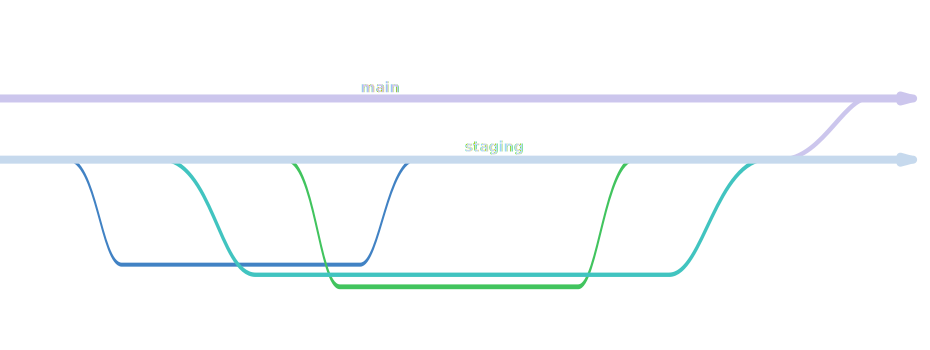
\includegraphics[width=0.8\textwidth]{img/branching}
    \centering
    \caption{Graphische Darstellung der Kombination aus git-flow und GitHub Flow}
    \label{fig:branchingModel}
\end{figure}

Das hier gezeigte Modell basiert relativ stark auf GitHub flow.
Es gibt einen Hauptbranch (Main), welcher zu jeder Zeit veröffentlichbar sein sollte.
Im Gegensatz zu GitHub flow ist dies allerdings nicht der main Branch, sondern ein staging Branch.
Dieser kann dann Nutzern als Beta-Version zur Verfügung gestellt werden.
So haben Nutzer die Möglichkeit neue Features sofort zu testen und direktes Feedback in den Entwicklungsprozess zurück zu bringen.
Im Gegensatz zu GitHub flow ist dies allerdings nicht der Branch, der in Production veröffentlicht wird.
Dafür gibt es den main branch, für den die gleichen Kriterien gelten wie für den Staging Branch.
Zudem darf auf den main branch allerdings nur eine getestete Version vom Staging Branch deployed werden.
Entwicklung sollte allerdings, genau wie bei GitHub flow, auf dem Main und Staging branch nicht stattfinden.
Hierfür werden für jedes Feature eigene Branches aufgemacht (dunkelblau, hellblau und grün in Abbildung~\ref{fig:branchingModel}).
Auf diesen werden alle commits gepushed, bis das feature bereit ist, in den Staging branch gemerged zu werden.
Dies bedeutet, dass das Feature vollständig funktioniert.
Sobald dieses Stadium erreicht ist, wird ein Pull Request in den Staging Branch erstellt.
Hiermit wird der Review Prozess eingeleitet.
Zunächst laufen natürlich alle automatisierten Tests und stellen die Codequalität und -funktionalität bestmöglich fest.
Im nächsten Schritt sollte der Merge Request von anderen Personen bestätigt werden und mögliche Fehler und Unstimmigkeiten sollten behoben werden.
Sobald diese Schritte durchlaufen sind, kann das Feature in den Staging Branch gemerged werden.
Nun rollt die Pipeline das Feature automatisch an alle Beta Nutzer aus, sodass eine realistische Testumgebung Feedback in den Entwicklungsprozess zurückspielen kann.
Unter der Annahme, dass hierbei keine Fehler auftreten kann man nun mit erhöhter Sicherheit und Stabilität den Staging Branch nach einem Pull Request in den Main Branch mergen, was ein Deployemnt für alle Nutzer auslöst.

Die Vorteile gegenüber GitHub flow liegen auf der Hand.
Ein Branchingmodell, welches nur minimal komplizierter ist, bringt eine stark erhöhte Stabilität im Programm, da Features zunächst an eine kleine Testgruppe ausgerollt wird, Feedback gesammelt wird und dieses erneut in den Entwicklungsprozess einfließen kann, bevor ein Feature an alle Nutzer ausgerollt wird.
Alle Vorteile von GitHub Flow gegenüber git-flow bleiben allerdings erhalten, weshalb dies immer noch ein exzellentes Modell für DevOps ist.

\subsection{Coding Guidelines/Code Architecture}\label{subsec:codingGuidelines/codeArchitecture}

Beginnen sollte man hier mit den Syntax- und Architekturtests.
Bevor die Funktionalität einer Software getestet wird, sollte man immer sicherstellen, dass die Architektur und Syntax den gewählten Konventionen entspricht.
Für die Bewertung der Position eines Schrittes in einer Pipeline gibt es mehrere ausschlaggebenden Punkte.
Wichtig sind aber vor allem, die Abhängigkeit zu anderen Schritten, sowie die Zeitkomplexität die mit dem Job einhergeht.
Nun wird auch schnell offensichtlich, warum dieser Schritt zu Beginn der Pipeline angeordnet sein sollte.
Es bestehen keine Abhängigkeiten zu anderen Jobs, weshalb dies problemfrei zu Beginn der Pipeline ausgeführt werden kann.
Außerdem sind Syntax- und Architekturtests in relativ kurzer Zeit auszuführen.
Dies ist erstrebenswert, da die Pipeline möglichst früh fehlschlagen sollte, wenn Fehler existieren, um unnötige Verzögerungen im Entwicklungsprozess zu vermeiden.
Zudem lassen sich Syntaxfehler zumeist schnell beheben, um die nächsten Schritte in der Pipeline erreichen zu können.